% =====================================================================
%  Chapitre 3 -- LSTM et GRU
%  Partie b : GRU, variantes, attention naissante, quiz, TP3
% =====================================================================

\begin{frame}{GRU : le LSTM allégé}
\begin{columns}[t]
\begin{column}{0.96\textwidth}
\begin{itemize}
  \item \textbf{Deux} portes au lieu de trois : update $z_t$ et reset $r_t$.
  \item Pas d'état de cellule séparé : $h_t$ fait double emploi.
  \item Équation : $h_t = (1 - z_t) \odot h_{t-1} + z_t \odot \tilde{h}_t$.
\end{itemize}
\begin{solbox}[Quand choisir ?]
Moins de paramètres, entraînement plus rapide : la GRU gagne souvent sur des
jeux de données modestes. Pour de longues dépendances, le LSTM garde l'avantage
--- mais mesurez les deux.
\end{solbox}
\end{column}
\end{columns}
% [fix] figure sortie
\end{frame}

\begin{frame}{GRU : le LSTM allégé --- la figure}\begin{center}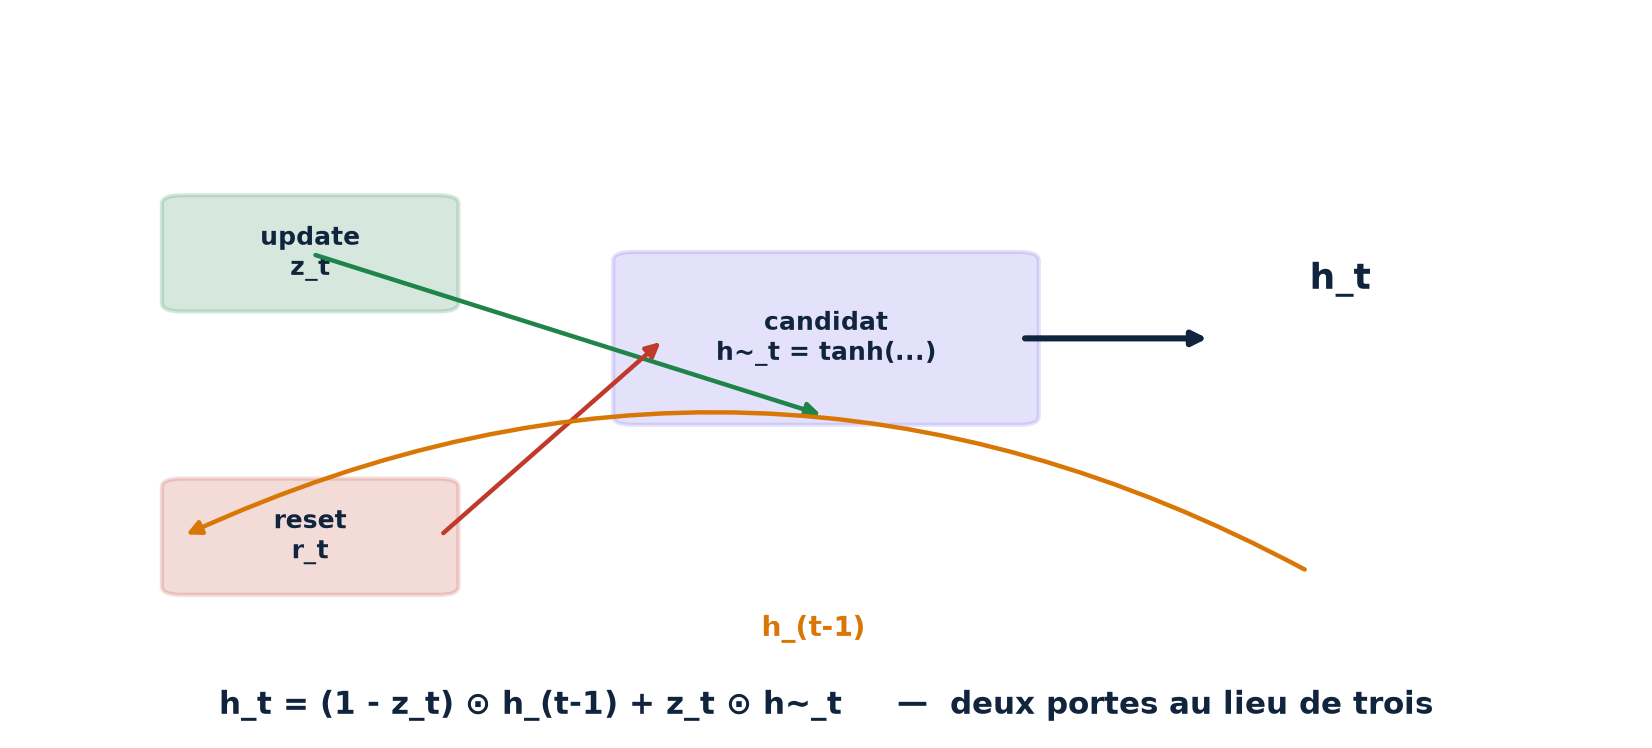
\includegraphics[width=.92\textwidth]{t05_gru.png}\end{center}\end{frame}

\begin{frame}{Le prix de la mémoire, en chiffres}
\begin{center}
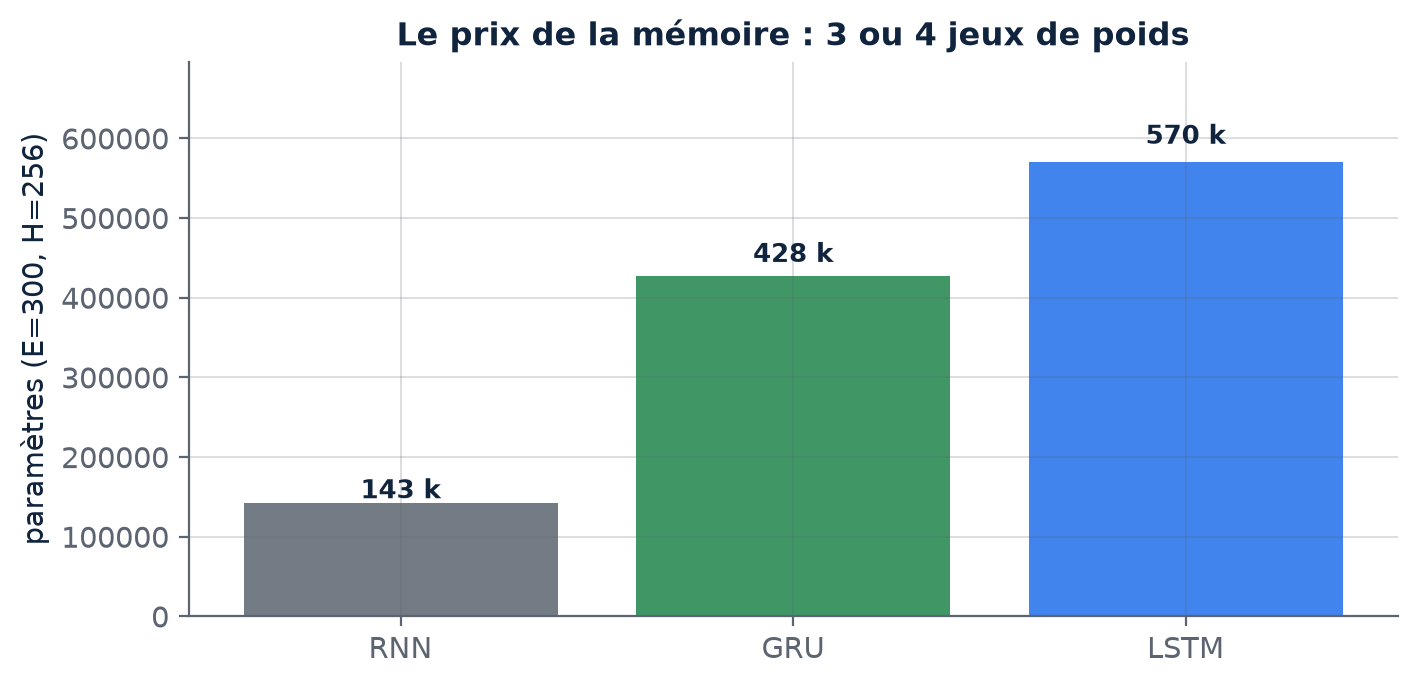
\includegraphics[width=0.8\textwidth]{t06_parametres.png}
\end{center}
\vspace{1mm}
\begin{itemize}
  \item LSTM : $4 \times (\text{entrées} \times H + H \times H) + 4H$.
  \item GRU : $3 \times (\text{entrées} \times H + H \times H) + 3H$.
  \item Avec $E = 300$, $H = 256$ : LSTM $\approx 573$ k, GRU $\approx 430$ k,
  RNN $\approx 143$ k paramètres.
\end{itemize}
\end{frame}

\begin{frame}{Bidirectionnel : lire dans les deux sens}
\begin{columns}[t]
\begin{column}{0.52\textwidth}
\centering
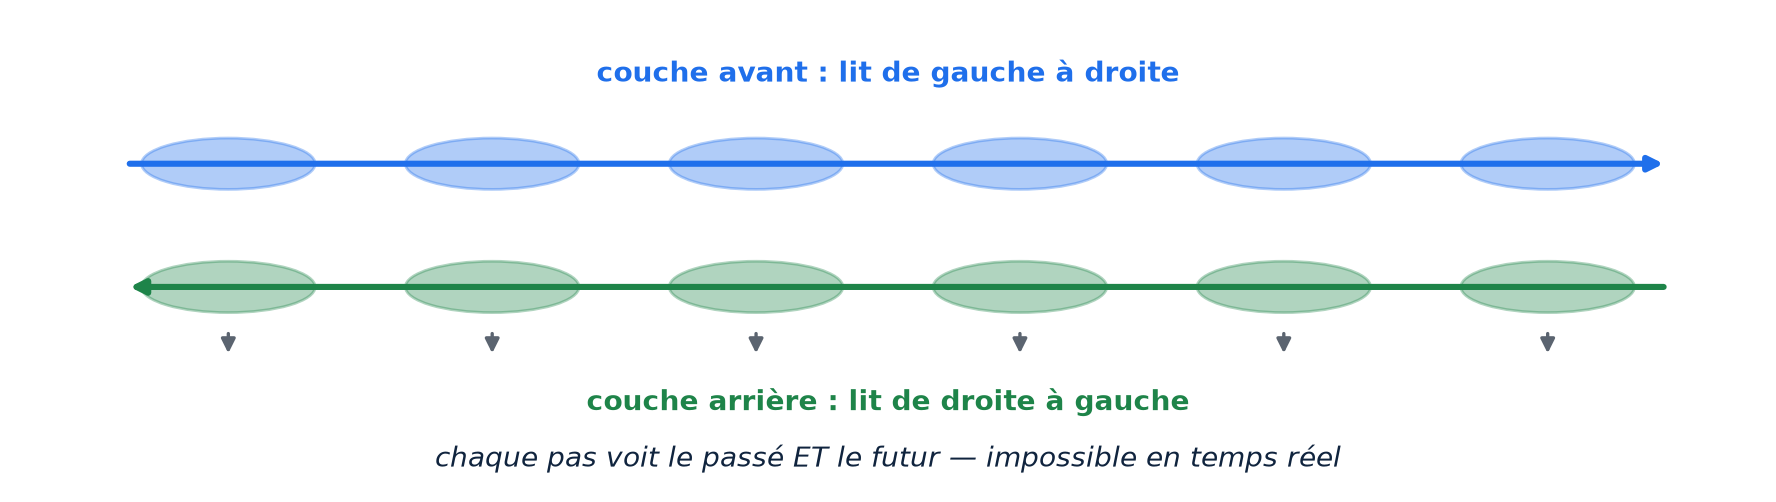
\includegraphics[width=\textwidth]{t07_bidirectionnel.png}
\end{column}
\begin{column}{0.44\textwidth}
\begin{itemize}
  \item Deux couches : une avant, une arrière ; leurs sorties se
  \textbf{concatènent}.
  \item Pour classer un mot, connaître \emph{ce qui suit} aide beaucoup.
\end{itemize}
\begin{wbox}[Le piège du temps réel]
Un modèle bidirectionnel ne peut pas prédire l'avenir : il a besoin de la
séquence \textbf{complète}. Interdit en streaming.
\end{wbox}
\end{column}
\end{columns}
\end{frame}

\begin{frame}{Empiler les couches}
\begin{columns}[t]
\begin{column}{0.48\textwidth}
\centering
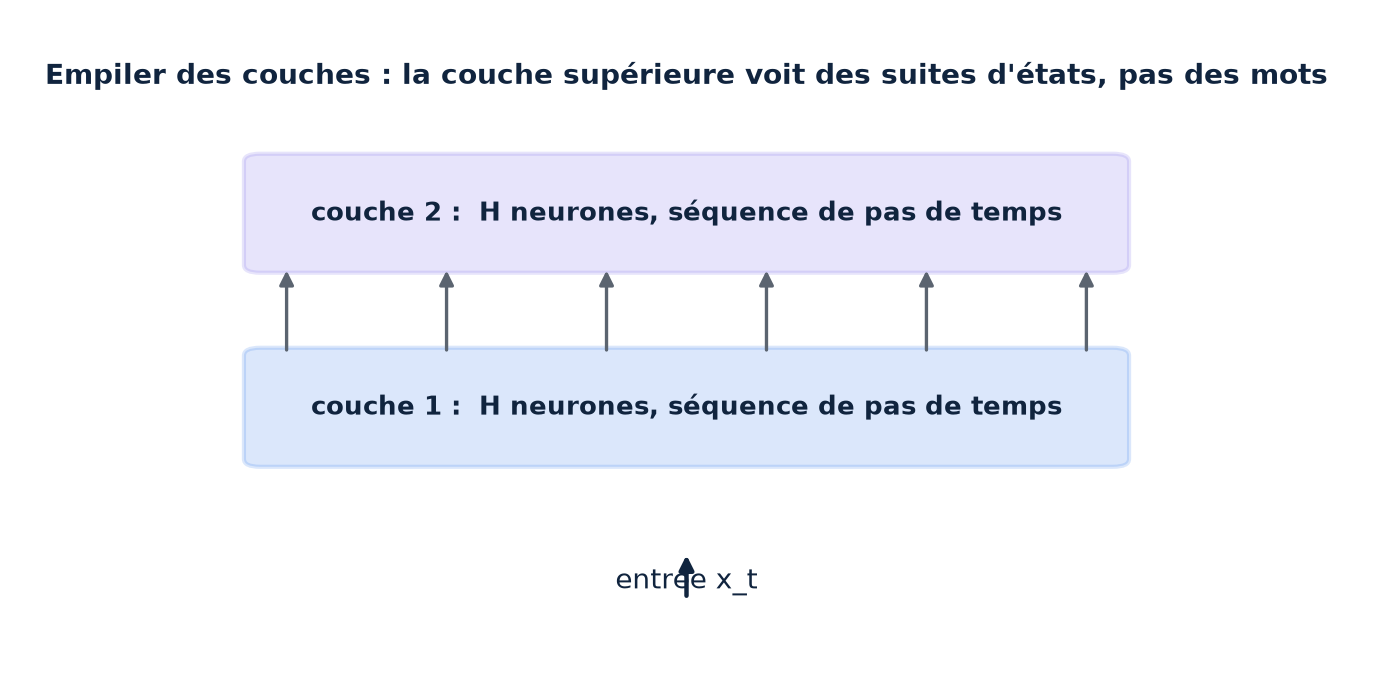
\includegraphics[width=0.9\textwidth]{t08_empilement.png}
\end{column}
\begin{column}{0.48\textwidth}
\begin{itemize}
  \item La sortie d'une couche récurrente est une \textbf{séquence} :
  on peut la donner à une autre couche récurrente.
  \item La couche 2 voit des états abstraits, pas des mots.
  \item Coût : temps de calcul et risque de surapprentissage --- deux couches
  suffisent presque toujours.
\end{itemize}
\end{column}
\end{columns}
\end{frame}

\begin{frame}{L'attention, en préfiguration}
\begin{columns}[t]
\begin{column}{0.96\textwidth}
\begin{itemize}
  \item Au lieu de compresser toute la séquence en un seul vecteur, le
  décodeur \textbf{regarde} tous les pas et pondère.
  \item Ici, pour décider, il pèse surtout « chat » et « tapis ».
\end{itemize}
\begin{kbox}[Pourquoi c'est une révolution]
L'attention résout le goulot d'étranglement du seq2seq --- et c'est la porte
d'entrée des \textbf{Transformers} (suite du programme).
\end{kbox}
\end{column}
\end{columns}
% [fix] figure sortie
\end{frame}

\begin{frame}{L'attention, en préfiguration --- la figure}\begin{center}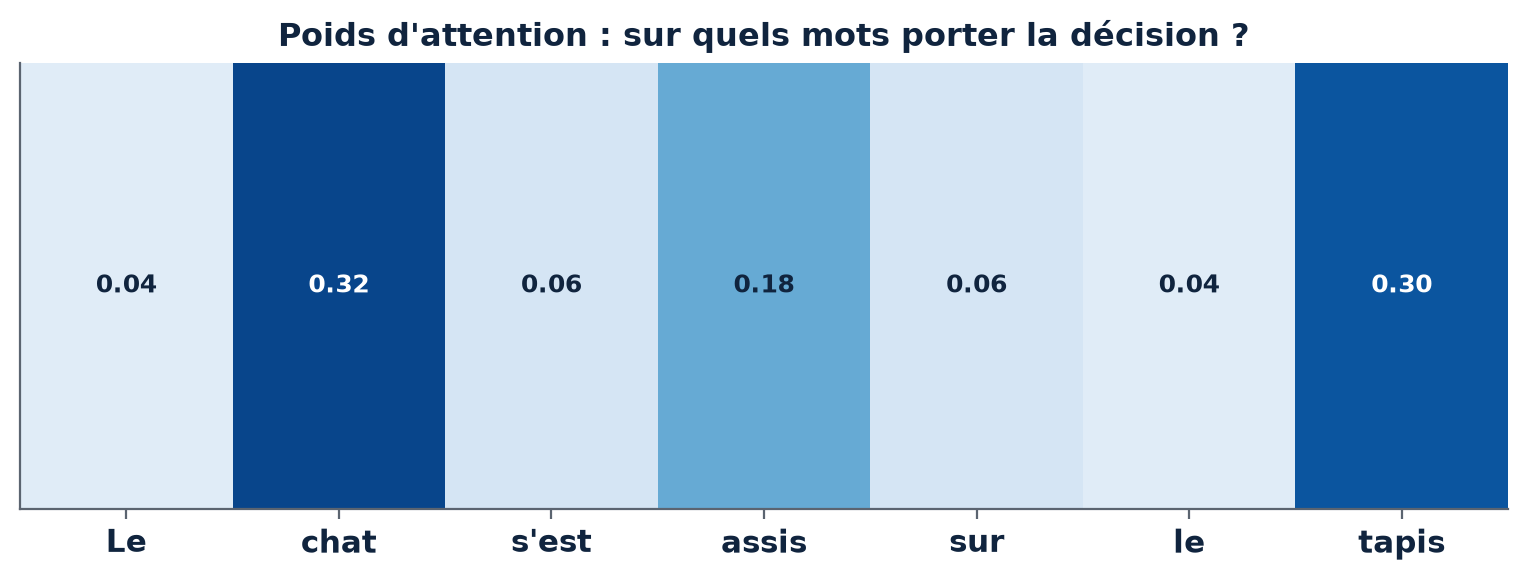
\includegraphics[width=.92\textwidth]{t09_attention.png}\end{center}\end{frame}

\begin{frame}{Quiz 4 --- LSTM, GRU et variantes}
\begin{qbox}[Question 1]
Combien de paramètres comporte une couche GRU, par rapport à un LSTM de même
taille ?
\begin{itemize}
  \item[(a)] les trois quarts \quad (b) les deux tiers \quad (c) autant
\end{itemize}
\end{qbox}
\begin{qbox}[Question 2]
Un LSTM bidirectionnel convient-il à un système de prédiction en temps réel ?
\begin{itemize}
  \item[(a)] oui, sans réserve \quad (b) non : il exige la séquence complète
  \quad (c) oui, si on le tronque
\end{itemize}
\end{qbox}
\begin{qbox}[Question 3]
Qu'apporte l'attention au seq2seq ?
\begin{itemize}
  \item[(a)] Elle accélère l'encodeur \quad (b) Elle supprime le goulot du
  vecteur unique \quad (c) Elle remplace le décodeur
\end{itemize}
\end{qbox}

% [fix] bloc deplace
\end{frame}
\begin{frame}{Quiz 4 --- LSTM, GRU et variantes (suite)}
\begin{solbox}[Réponses]
\textbf{1.} (b) : trois jeux de poids contre quatre. \quad
\textbf{2.} (b) : la couche arrière lit la fin. \quad
\textbf{3.} (b) : le décodeur consulte tous les pas de la source.
\end{solbox}
\end{frame}

\begin{frame}{À retenir et TP}
\begin{kbox}[Les trois idées du chapitre 3]
\begin{enumerate}
  \item Le LSTM protège l'information par un \textbf{convoyeur} :
  $C_t = f_t \odot C_{t-1} + i_t \odot \tilde{C}_t$.
  \item La porte d'oubli proche de 1 maintient le gradient : $0{,}99^{30}
  = 0{,}74$ au lieu de $2 \times 10^{-8}$.
  \item GRU = deux portes, moins de paramètres ; bidirectionnel = les deux sens
  mais pas de temps réel.
\end{enumerate}
\end{kbox}
\vspace{1.5mm}
\begin{abox}[TP3 : \file{notebooks/TP3_LSTM_GRU_sentiment.ipynb}]
Comparer RNN, LSTM et GRU sur la classification de critiques, avec et sans
bidirectionnel. Durée : \textbf{2 h} · barème : \textbf{10 points}.
\end{abox}
\end{frame}
